% Figure 2: Defect Density Pipeline - From Discrete to Curvature to Arrow of Time
% Standalone TikZ figure for BP3
\documentclass[tikz,border=5pt]{standalone}
\usepackage{tikz}
\usepackage{amsmath,amssymb}
\usetikzlibrary{shapes.geometric,arrows.meta,positioning,decorations.pathmorphing,calc,patterns,shadings}

\begin{document}
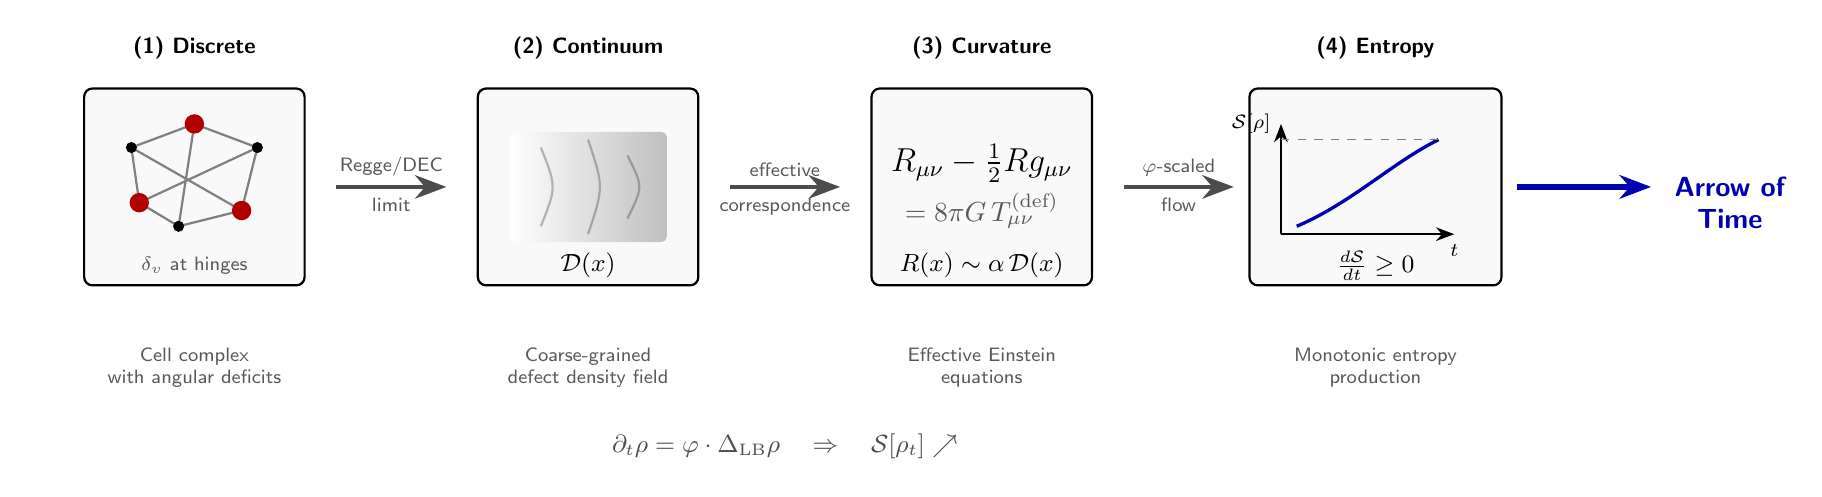
\begin{tikzpicture}[
    box/.style={draw=black, thick, rounded corners=3pt, minimum width=2.8cm, minimum height=2cm, align=center, fill=gray!5},
    arrow/.style={-{Stealth[length=4mm, width=3mm]}, very thick, black!70},
    label/.style={font=\small\sffamily},
    sublabel/.style={font=\scriptsize\sffamily, gray!70!black},
    mathlabel/.style={font=\small},
    stage/.style={font=\footnotesize\sffamily\bfseries, above}
]

% === STAGE 1: Discrete Complex with Defects ===
\begin{scope}[shift={(0,0)}]
    \node[box, minimum height=2.5cm] (box1) at (0,0) {};
    \node[stage] at (0,1.5) {(1) Discrete};

    % Draw a small network with defect points
    \coordinate (n1) at (-0.8,0.5);
    \coordinate (n2) at (0,0.8);
    \coordinate (n3) at (0.8,0.5);
    \coordinate (n4) at (0.6,-0.3);
    \coordinate (n5) at (-0.2,-0.5);
    \coordinate (n6) at (-0.7,-0.2);

    % Edges
    \draw[gray, thick] (n1) -- (n2) -- (n3) -- (n4) -- (n5) -- (n6) -- (n1);
    \draw[gray, thick] (n2) -- (n5);
    \draw[gray, thick] (n1) -- (n4);
    \draw[gray, thick] (n3) -- (n6);

    % Vertices (normal)
    \fill[black] (n1) circle (2pt);
    \fill[black] (n3) circle (2pt);
    \fill[black] (n5) circle (2pt);

    % Defect vertices (highlighted)
    \fill[red!70!black] (n2) circle (3.5pt);
    \fill[red!70!black] (n4) circle (3.5pt);
    \fill[red!70!black] (n6) circle (3.5pt);

    % Label
    \node[sublabel] at (0,-1) {$\delta_v$ at hinges};
\end{scope}

% Arrow 1->2
\draw[arrow] (1.8,0) -- node[above, sublabel] {Regge/DEC} node[below, sublabel] {limit} (3.2,0);

% === STAGE 2: Coarse-grained Defect Field ===
\begin{scope}[shift={(5,0)}]
    \node[box, minimum height=2.5cm] (box2) at (0,0) {};
    \node[stage] at (0,1.5) {(2) Continuum};

    % Shaded density field (gradient)
    \shade[left color=white, right color=gray!50, rounded corners=2pt] (-1,-0.7) rectangle (1,0.7);

    % Contour lines
    \draw[gray!60, thick] (-0.6,-0.5) .. controls (-0.4,0) .. (-0.6,0.5);
    \draw[gray!70, thick] (0,-0.6) .. controls (0.2,0) .. (0,0.6);
    \draw[gray!80, thick] (0.5,-0.4) .. controls (0.7,0) .. (0.5,0.4);

    % Label
    \node[mathlabel] at (0,-1) {$\mathcal{D}(x)$};
\end{scope}

% Arrow 2->3
\draw[arrow] (6.8,0) -- node[above, sublabel] {effective} node[below, sublabel] {correspondence} (8.2,0);

% === STAGE 3: Curvature ===
\begin{scope}[shift={(10,0)}]
    \node[box, minimum height=2.5cm] (box3) at (0,0) {};
    \node[stage] at (0,1.5) {(3) Curvature};

    % Symbolic curvature representation (not a bending grid!)
    % Use abstract symbols
    \node[font=\large] at (0,0.3) {$R_{\mu\nu} - \tfrac{1}{2}Rg_{\mu\nu}$};
    \node[font=\normalsize, gray!70!black] at (0,-0.3) {$= 8\pi G\, T_{\mu\nu}^{(\text{def})}$};

    % Label
    \node[mathlabel] at (0,-1) {$R(x) \sim \alpha\,\mathcal{D}(x)$};
\end{scope}

% Arrow 3->4
\draw[arrow] (11.8,0) -- node[above, sublabel] {$\varphi$-scaled} node[below, sublabel] {flow} (13.2,0);

% === STAGE 4: Entropy and Arrow of Time ===
\begin{scope}[shift={(15,0)}]
    \node[box, minimum height=2.5cm, minimum width=3.2cm] (box4) at (0,0) {};
    \node[stage] at (0,1.5) {(4) Entropy};

    % Entropy increase graph
    \draw[-{Stealth}, thick] (-1.2,-0.6) -- (-1.2,0.8) node[left, font=\scriptsize] {$\mathcal{S}[\rho]$};
    \draw[-{Stealth}, thick] (-1.2,-0.6) -- (1,-0.6) node[below, font=\scriptsize] {$t$};

    % Monotonically increasing curve
    \draw[blue!70!black, very thick] (-1,-0.5) .. controls (-0.3,-0.2) and (0.2,0.3) .. (0.8,0.6);

    % Equilibrium asymptote (dashed)
    \draw[gray, dashed] (-1.2,0.6) -- (0.9,0.6);

    % Label
    \node[mathlabel] at (0,-1) {$\tfrac{d\mathcal{S}}{dt} \geq 0$};
\end{scope}

% === Final Arrow: Arrow of Time ===
\draw[arrow, blue!70!black, line width=2pt] (16.8,0) -- (18.5,0);
\node[font=\sffamily\bfseries, blue!70!black] at (19.5,0) {Arrow of};
\node[font=\sffamily\bfseries, blue!70!black] at (19.5,-0.4) {Time};

% === Bottom annotations ===
\node[sublabel, text width=4cm, align=center] at (0,-2.3) {Cell complex\\with angular deficits};
\node[sublabel, text width=4cm, align=center] at (5,-2.3) {Coarse-grained\\defect density field};
\node[sublabel, text width=4cm, align=center] at (10,-2.3) {Effective Einstein\\equations};
\node[sublabel, text width=4cm, align=center] at (15,-2.3) {Monotonic entropy\\production};

% === Flow equation at bottom ===
\node[mathlabel, gray!60!black] at (7.5,-3.3) {
$\partial_t \rho = \varphi \cdot \Delta_{\text{LB}} \rho \quad\Rightarrow\quad \mathcal{S}[\rho_t] \nearrow$
};

\end{tikzpicture}
\end{document}
